\section{Methodology}~\label{sec:methodology}

The methodology for generating descriptors from a learning process based on the fusion of images and point clouds is divided into several stages: The first stage corresponds to the adjustment or preprocessing of the point cloud so that it can be projected onto the panoramic image. Then, based on the model presented by \cite{Lin2025}, the point cloud and the images are fed into the network to obtain perceptual features from both modalities individually through feature fusion using attention-based models.
Next, the projected point cloud is transformed into the 3D space using sparse convolutions within a refinement module to optimize the segmentation produced by both modalities. Finally, a trainable global descriptor is constructed, which transforms the multimodal 3D features into a discriminative embedding for the identification of the objects present in the scene.

\subsection{Panoramic Images Generation}~\label{subsec:panoramic-image-generation}

For comprehensive scene understanding and environmental awareness, the use of panoramic images offers significant advantages over single-camera setups, particularly in outdoor and large-scale autonomous perception scenarios. The panoramic representation of our multi-sensor system provides a 180-degree field of view, enabling the system to capture in front of the vehicle spatial context of a scene in a single frame. 

\newpage

\begin{strip}
	\centering
	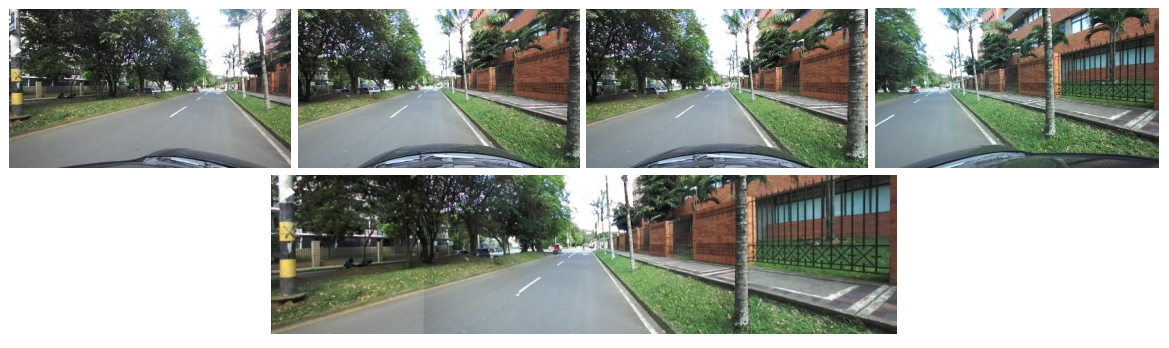
\includegraphics[width=\linewidth]{Figures/Stitching images_to_panoramic_uao.pdf} 	
	\captionof{figure}{Panoramic Image Generation via Multi-Camera Homography Alignment and Stitching.}	
	\label{fig:panoramic-image-generation}
\end{strip}

This holistic perception reduces blind spots and allows the model to reason about long-range spatial relationships between objects that would otherwise be distributed across multiple independent camera views. By observing the entire surrounding environment simultaneously, the system gains a more coherent representation of scene layout, object distribution, and structural continuity. \\
In contrast, single-camera images are inherently limited by their narrower field of view, which can restrict contextual reasoning and lead to partial observations of large structures such as buildings, intersections, or dynamic objects. This limitation may require additional multi-view fusion strategies to approximate a global understanding of the environment. Panoramic imagery, therefore, naturally supports richer contextual modeling, improved spatial completeness, and more consistent global representations of complex scenes.
The process begins with feature extraction, where salient keypoints and corresponding binary descriptors are detected using the ORB~\cite{Rublee2011} algorithm. ORB is selected due to its computational efficiency and robustness to rotation and illumination changes, making it suitable for real-time multi-camera applications. The input images have an initial spatial resolution of 1280 × 720 pixels, providing sufficient detail for reliable keypoint detection and matching.
Following feature extraction, a keypoint matching stage is performed between overlapping image pairs. Descriptor correspondences are established using a nearest-neighbor search strategy, typically based on Hamming distance due to ORB’s binary descriptors. These correspondences provide the geometric constraints necessary for estimating the transformation between views. \\

Next, a homography matrix is computed using the matched keypoints. To ensure robustness against incorrect correspondences (outliers), the homography is estimated using the RANSAC (Random Sample Consensus) algorithm. RANSAC iteratively selects minimal subsets of correspondences to compute candidate homographies and retains the solution that maximizes inlier consistency, thereby improving geometric accuracy.
Once the homography matrix is obtained, a perspective warping step is applied. One image is projected onto the coordinate frame of the reference image using a perspective transformation, aligning the overlapping regions into a common plane. This warping compensates for viewpoint differences between cameras under the planar scene assumption.
Finally, after geometric alignment and stitching, the resulting composite image undergoes cropping to remove redundant regions and boundary artifacts. The final panoramic output has a spatial resolution of 908 × 230 pixels, producing a compact, horizontally extended representation suitable for downstream perception tasks. This process is showed in Fig.~\ref{fig:panoramic-image-generation}.

\subsection{Preprocessing of the Point Cloud}~\label{subsec:lidar-preprocessing}

Several strategies can be employed to project 3D point clouds onto the image domain, including perspective, cylindrical~\cite{Kang2019RobustCP}, and spherical projections~\cite{HeYingshen2020}. The selection of the projection model is strongly influenced by the imaging geometry, sensor configuration, and especially the field of view of the camera system. In scenarios involving panoramic images with a wide angular coverage, spherical projection offers a more consistent geometric formulation than conventional perspective projection. Unlike perspective models, which are inherently limited to narrower fields of view and may introduce severe distortions at large viewing angles, spherical parameterization maintains the angular continuity of the scene by directly mapping LiDAR points according to their azimuth and elevation angles. This property ensures a more uniform spatial correspondence between 3D points and image pixels, thereby improving the stability of cross-modal alignment and facilitating more reliable multimodal feature fusion.
To perform the spherical projection as depicted in Fig.~\ref{fig:spherical-projection}, we first convert the Cartesian coordinates of the LiDAR points into spherical coordinates. Each point in the point cloud is represented by its range $r$, azimuth angle $\theta$, and elevation angle $\phi$. These type of images are dependent on the LiDAR's design parameters. It is important to know the vertical field of view (FOV) and the number of channels of the LiDAR to determine the resolution of the projected image. The vertical FOV defines the range of elevation angles that the LiDAR can capture, while the number of channels determines how many discrete elevation angles are sampled within that FOV. 

\newpage

\begin{strip}
	\centering
	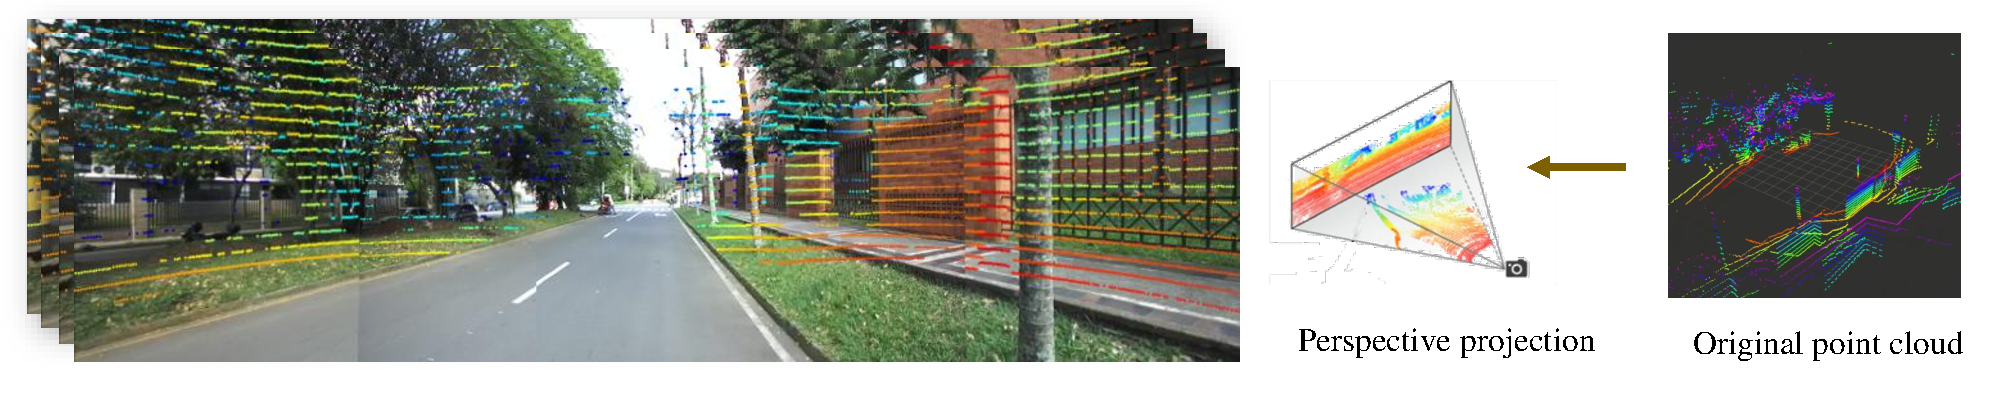
\includegraphics[width=\linewidth]{Figures/Spherical_point_cloud_projection.pdf} 	
	\captionof{figure}{Spherical Projection of LiDAR Point Cloud onto the Panoramic Image Plane.}	
	\label{fig:spherical-projection}
\end{strip}

This means that each channel corresponds to a specific elevation angle, and the point cloud can be projected onto a 2D image where each pixel corresponds to a specific azimuth and elevation angle. The horizontal resolution is determined by the azimuthal sampling, which is typically uniform across the 360-degree horizontal field of view. 
We compurte the depth of each point in the point cloud as the Euclidean distance from the LiDAR sensor to the point, which can be calculated using the formula:
\begin{equation}
    r = \sqrt{x^2 + y^2 + z^2}  
\end{equation}
where $x$, $y$, and $z$ are the Cartesian coordinates of the point.
Then, we calculate the azimuth angle $\theta$ and elevation angle $\phi$ for each point using the following formulas:
\begin{equation}
    \phi = \tan^{-1}\left(\frac{y}{x} \right) 
\end{equation}
\begin{equation}    \theta = \sin^{-1}\left(\frac{z}{r}\right)
\end{equation}
Afterward, each of the angles needs to be normalized to range between $[0,1]$, and then remapped to the perspective ranges of $[0, W]$ for yaw and $[0, H]$ for pitch, where $W$ and $H$ are the width and height of the projected image, respectively. The remapping can be performed using the following equations:

\begin{equation}    
    u = 0.5 \cdot \frac{\phi}{\pi} \cdot W
\end{equation}
\begin{equation}    
    v = \left(1.0 - \left( \frac{\theta + |fov_{down}|}{fov} \right) \right)\cdot H
\end{equation}
where $fov$ is the total vertical field of view of the LiDAR, and $fov_{down}$ is the downward vertical field of view. The resulting coordinates $(u, v)$ represent the pixel location in the projected image corresponding to each point in the point cloud. This process effectively transforms the 3D spatial information from the LiDAR into a 2D representation that can be easily fused with the panoramic image data for subsequent feature extraction and descriptor generation.

\subsection{Deep Multi-Modal Semantic Segmentation}~\label{subsec:multi-modal-semantic-segmentation}